% D^2 as a CW complex with 2+2+1 cells: two 0-cells, two 1-cells, one 2-cell.
% Source: book/tex/topology/constructions.tex (§ CW complexes).
\documentclass[border=2mm]{standalone}
\usepackage{tikz}
\begin{document}
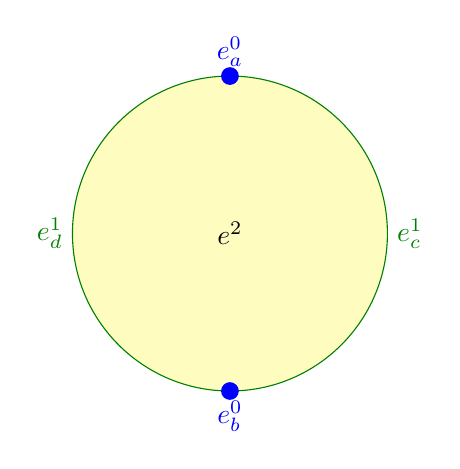
\begin{tikzpicture}[scale=2]
  \fill[yellow!25] (0,0) circle (1);
  \draw[green!50!black] (0,0) circle (1);
  \fill[blue] (0,1) circle (1.6pt) node[above,blue] {$e_a^0$};
  \fill[blue] (0,-1) circle (1.6pt) node[below,blue] {$e_b^0$};
  \node[green!50!black,right] at (1,0) {$e_c^1$};
  \node[green!50!black,left] at (-1,0) {$e_d^1$};
  \node at (0,0) {$e^2$};
\end{tikzpicture}
\end{document}
